
\section{Computer Algebra Representation}
\label{sec:car}

Our computer algebra representation is based on mathematical expression trees, which are hierarchies of expression instances. An expressions can be either a basic primitive, such as a number, variable or special symbol, such as the Kronecker delta or imaginary number. Other expression types, such as integrals, derivatives, sums, products and functions, build the hierarchy by referencing child expressions.

Our framework further provides manipulators, which can be executed on expressions. We implemented all manipulations required to derive the $P_N$-equations. This includes application of the distributive law, substitution, constant folding, reordering of nested integrals, application of identities up to more complex operations, such as factorization of unknowns and discretization of spatial variables. The derivation steps of the real-valued $P_N$-equations in the supplemental material were all carried out using our framework.

\begin{figure}[h]
%\vspace{1in}
\centering
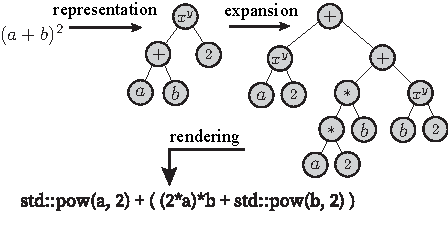
\includegraphics[width=0.9\columnwidth]{figures/fig_car.pdf}
\vspace{-0.16in}
\icaption{Our computer algebra framework allows to represent equations as mathematical expressions trees. It further provides a set of functions for manipulating the tree according to valid mathematical operations, such as the binomial expansion above. Frontends allow generation of source code from the expression tree.}
\label{fig:staggeredgrid}
\end{figure}

%Our computer algebra framework allows to represent equations as mathematical expressions trees. It further provides a set of functions, which manipulate the tree according to valid mathematical operations, such as the binomial expansion above. Rendering frontends allow generation of source or code from the expression tree.

Finally, frontends allow rendering the expression tree into different forms. We implemented frontends for rendering expression trees to \LaTeX~and C++ source code. The equations in the supplemental material were almost all rendered by the former. The latter was used for generating the stencil code used by our solver.


Note that our framework is different from a computer algebra system (CAS), such as Mathematica. While these systems probably use similar representations internally, they are aimed at finding answers to mathematical problems and have not been designed to allow application of custom manipulation passes on the expression tree. Our framework has been written solely for that purpose. It only deals with representation and manipulation of mathematical expressions and therefore is very lightweight and easy to use.
